\begin{comment}


\begin{center}
\thispagestyle{empty}
%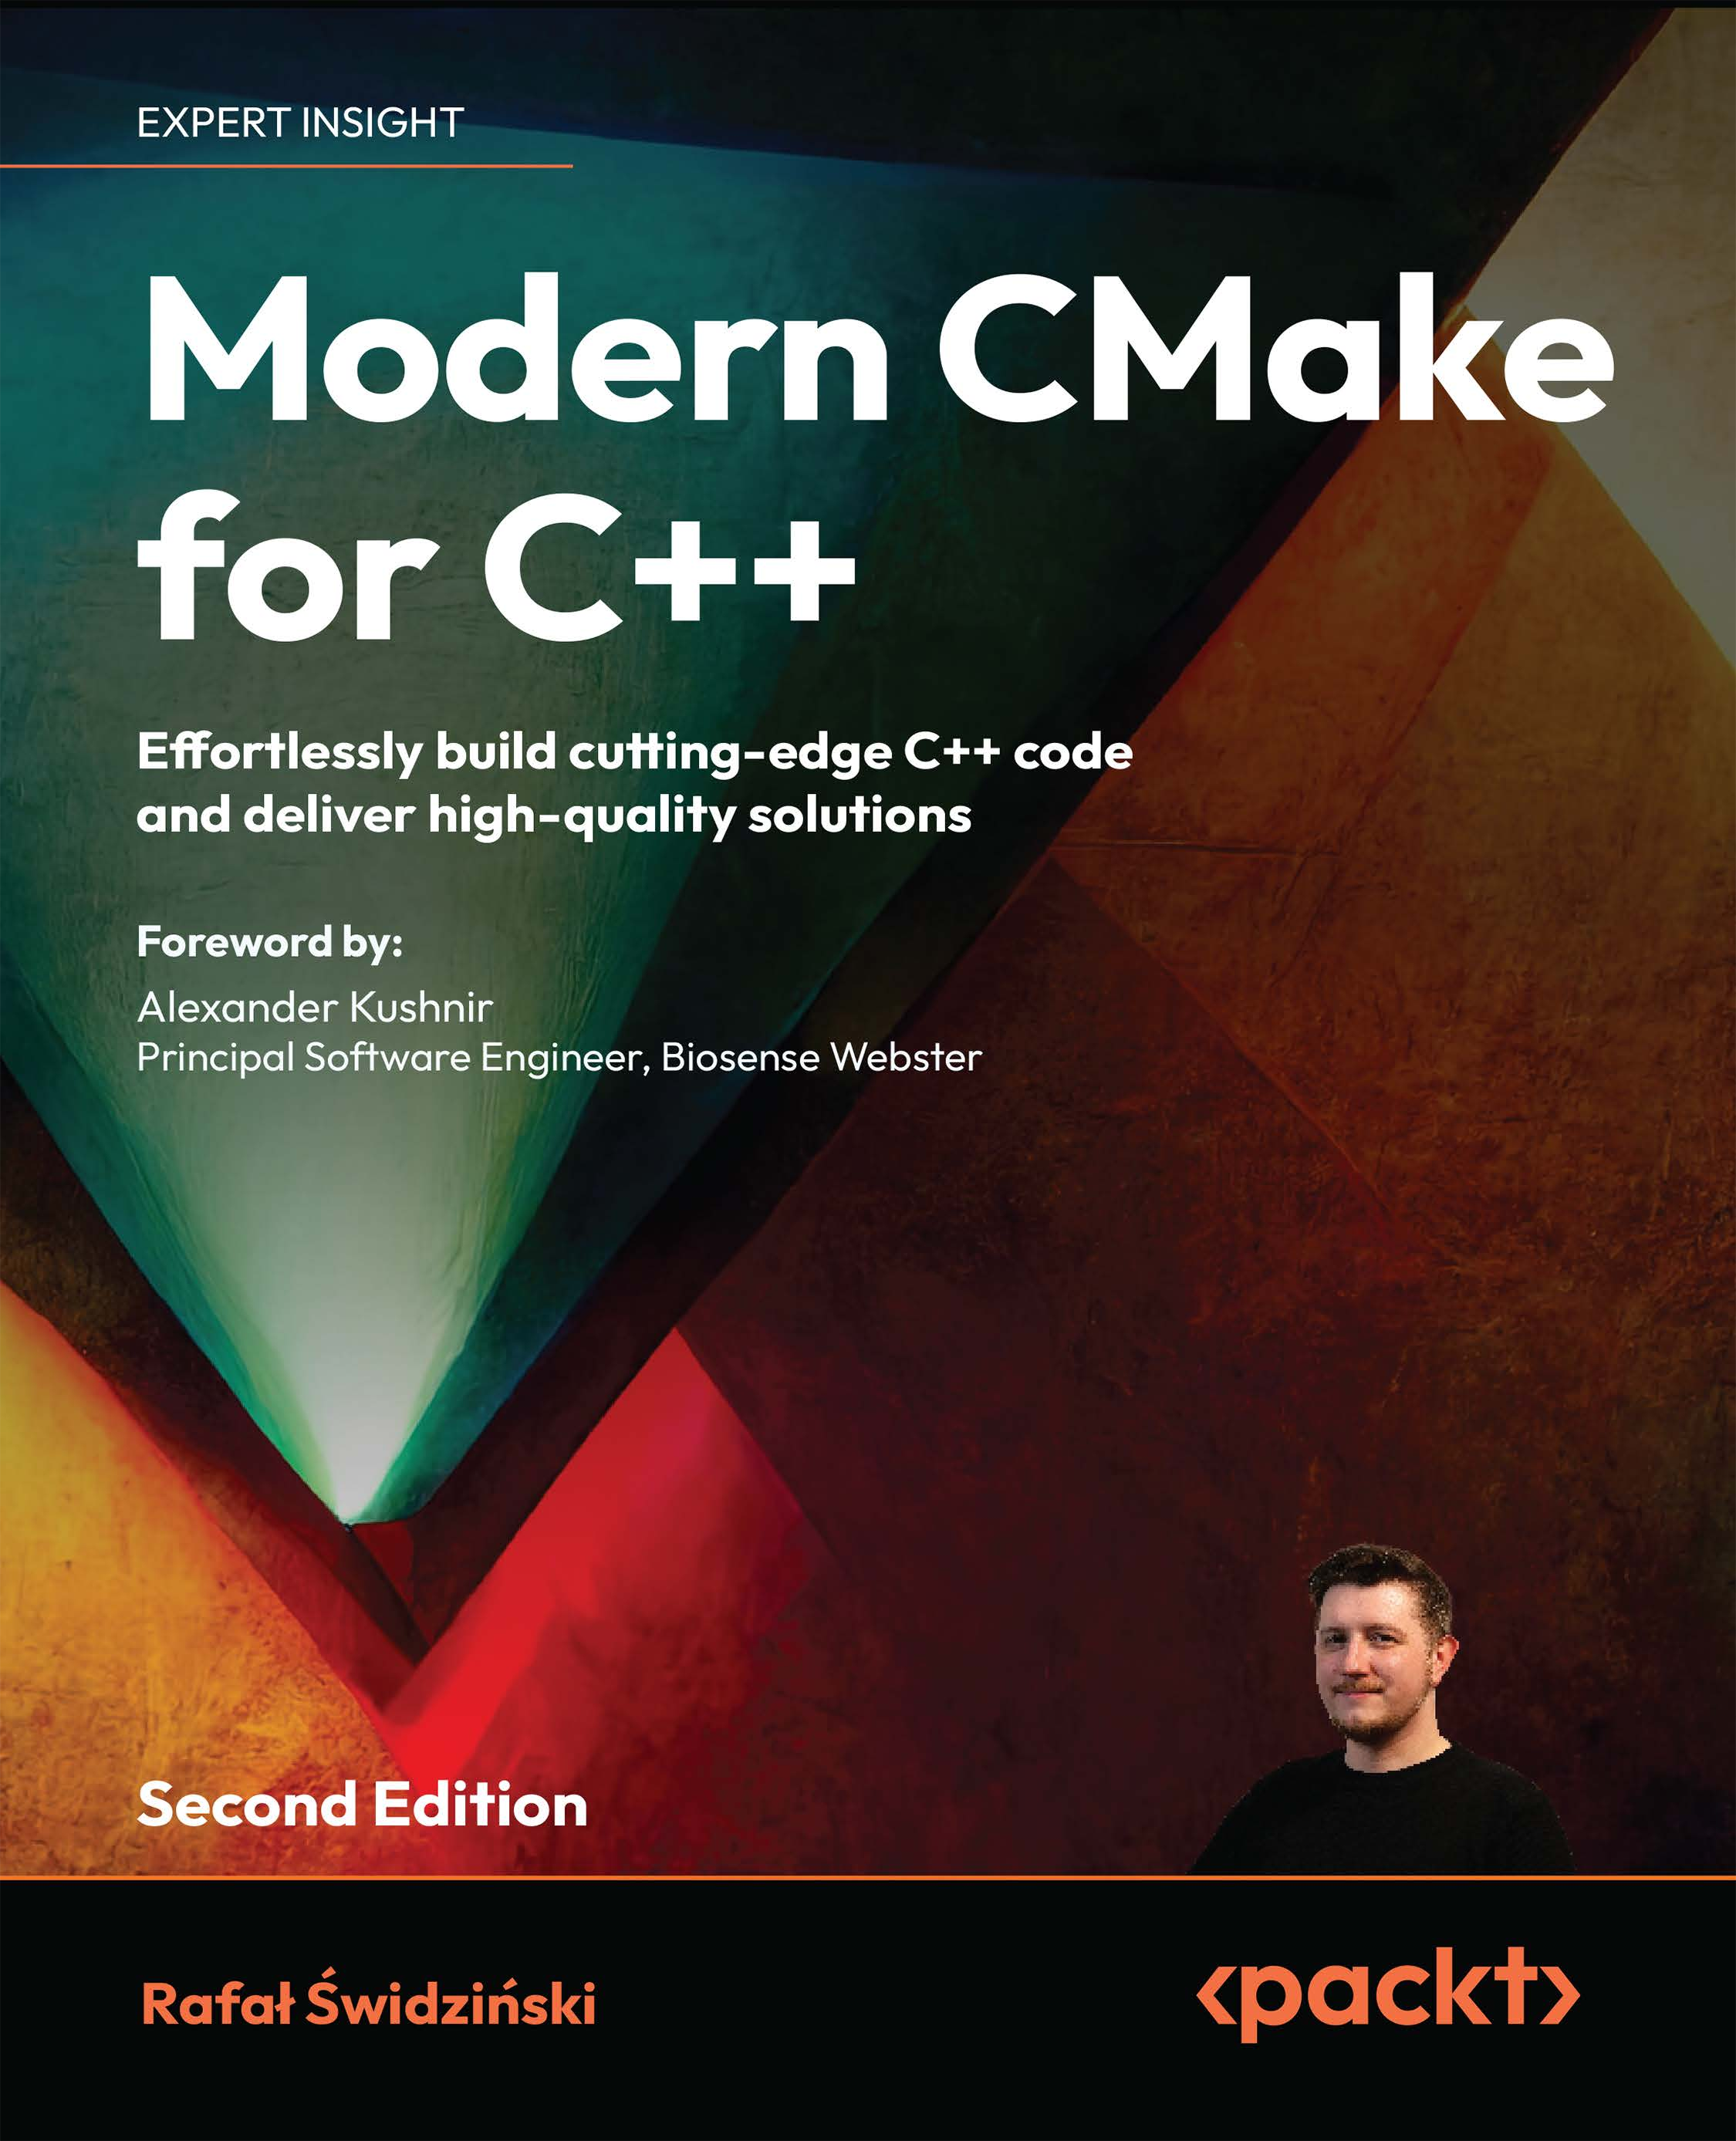
\includegraphics[width=\textwidth,height=\textheight,keepaspectratio]{cover.png}
\begin{tikzpicture}[remember picture, overlay, inner sep=0pt]
\node at (current page.center)
{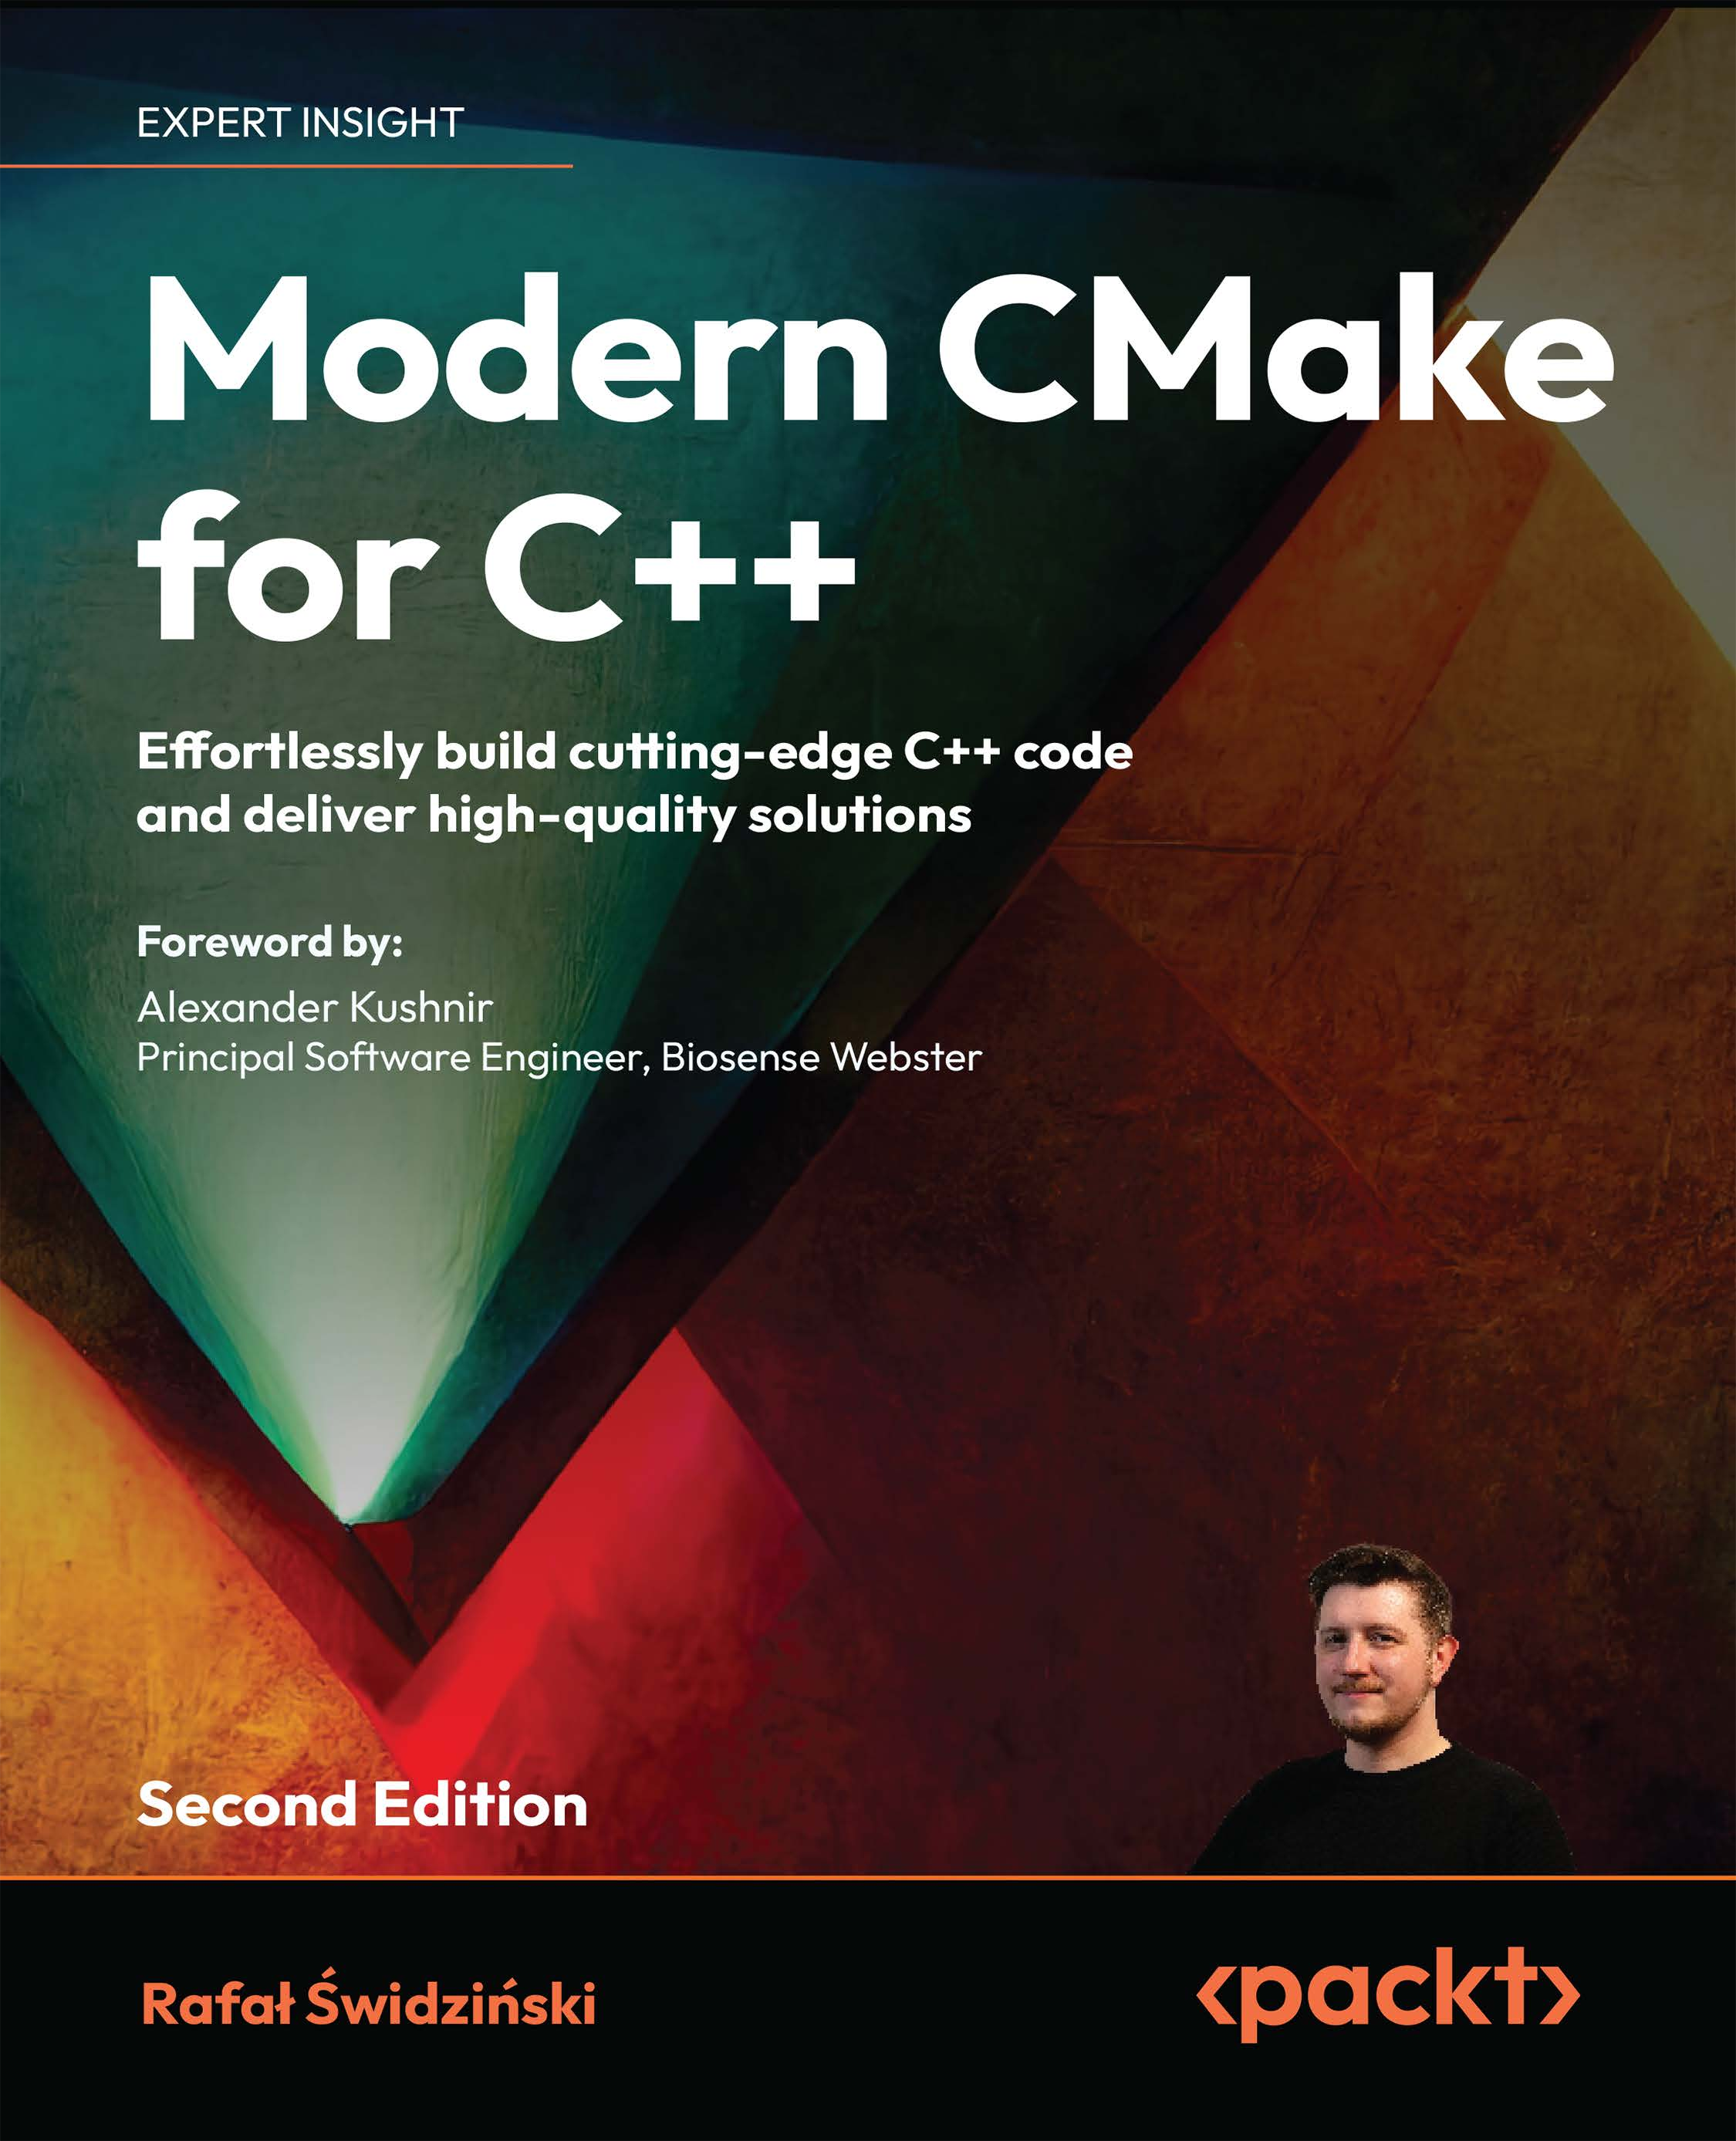
\includegraphics[width=\paperwidth, keepaspectratio=false]{cover.png}};
\end{tikzpicture}
\newpage
\thispagestyle{empty}
\huge
\textbf{Modern CMake for C++ - Second Edition}
\\[9pt]
{\Large Effortlessly build cutting-edge C++ code and deliver high-quality solutions}
\\[9pt]
\normalsize
作者: Rafał Świdziński
\\[8pt]
\normalsize
译者:\href{https://github.com/xiaoweiChen/Modern-CMake-for-Cpp-2ed}{陈晓伟}
\\[8pt]
\end{center}

\newpage

\pagestyle{empty}
\tableofcontents
\newpage

\setsecnumdepth{section}

\myPart{}{序}{content/Foreword.tex}
\newpage

\myPart{}{关于作者}{content/Contributors.tex}
\newpage

\myPart{}{关于评审}{content/Reviewers.tex}
\newpage

\myPart{}{前言}{content/Preface.tex}
\newpage

\myChapter{第1章}{First Steps with CMake}{content/chapter1/0.tex}
\mySubsection{1.1.}{Technical requirements}{content/chapter1/1.tex}
\mySubsection{1.2.}{Understanding the basics}{content/chapter1/2.tex}
\mySubsection{1.3.}{Installing CMake on different platforms}{content/chapter1/3.tex}
\mySubsection{1.4.}{Mastering the command line}{content/chapter1/4.tex}
\mySubsection{1.5.}{Navigating project directories and files}{content/chapter1/5.tex}
\mySubsection{1.6.}{Discovering scripts and modules}{content/chapter1/6.tex}
\mySubsection{1.7.}{总结}{content/chapter1/7.tex}
\mySubsection{1.8.}{扩展阅读}{content/chapter1/8.tex}
\newpage

\myChapter{第2章}{The CMake Language}{content/chapter2/0.tex}
\mySubsection{2.1.}{Technical requirements}{content/chapter2/1.tex}
\mySubsection{2.2.}{The basics of the CMake language syntax}{content/chapter2/2.tex}
\mySubsection{2.3.}{Working with variables}{content/chapter2/3.tex}
\mySubsection{2.4.}{Using lists}{content/chapter2/4.tex}
\mySubsection{2.5.}{Understanding control structures in CMake}{content/chapter2/5.tex}
\mySubsection{2.6.}{Exploring the frequently used commands}{content/chapter2/6.tex}
\mySubsection{2.7.}{总结}{content/chapter2/7.tex}
\mySubsection{2.8.}{扩展阅读}{content/chapter2/8.tex}
\newpage

\myChapter{第3章}{Using CMake in Popular IDEs}{content/chapter3/0.tex}
\mySubsection{3.1.}{Getting to know IDEs}{content/chapter3/1.tex}
\mySubsection{3.2.}{Starting with the CLion IDE}{content/chapter3/2.tex}
\mySubsection{3.3.}{Starting with Visual Studio Code}{content/chapter3/3.tex}
\mySubsection{3.4.}{Starting with the Visual Studio IDE}{content/chapter3/4.tex}
\mySubsection{3.5.}{总结}{content/chapter3/5.tex}
\mySubsection{3.6.}{扩展阅读}{content/chapter3/6.tex}
\newpage
\end{comment}
\myChapter{第4章}{Setting Up Your First CMake Project}{content/chapter4/0.tex}
\mySubsection{4.1.}{Technical requirements}{content/chapter4/1.tex}
\mySubsection{4.2.}{Understanding the basic directives and commands}{content/chapter4/2.tex}
\mySubsection{4.3.}{Partitioning your project}{content/chapter4/3.tex}
\mySubsection{4.4.}{Thinking about the project structure}{content/chapter4/4.tex}
\mySubsection{4.5.}{Scoping the environment}{content/chapter4/5.tex}
\mySubsection{4.6.}{Configuring the toolchain}{content/chapter4/6.tex}
\mySubsection{4.7.}{Disabling in-source builds}{content/chapter4/7.tex}
\mySubsection{4.8.}{总结}{content/chapter4/8.tex}
\mySubsection{4.9.}{扩展阅读}{content/chapter4/9.tex}
\newpage
\begin{comment}
\myChapter{第5章}{Working with Targets}{content/chapter5/0.tex}
\mySubsection{5.1.}{Technical requirements}{content/chapter5/1.tex}
\mySubsection{5.2.}{Understanding the concept of a target}{content/chapter5/2.tex}
\mySubsection{5.3.}{Writing custom commands}{content/chapter5/3.tex}
\mySubsection{5.4.}{总结}{content/chapter5/4.tex}
\mySubsection{5.5.}{扩展阅读}{content/chapter5/5.tex}
\newpage

\myChapter{第6章}{Using Generator Expressions}{content/chapter6/0.tex}
\mySubsection{6.1.}{Technical requirements}{content/chapter6/1.tex}
\mySubsection{6.2.}{What are generator expressions?}{content/chapter6/2.tex}
\mySubsection{6.3.}{Learning the basic rules of general expression syntax}{content/chapter6/3.tex}
\mySubsection{6.4.}{Conditional expansion}{content/chapter6/4.tex}
\mySubsection{6.5.}{Querying and transforming}{content/chapter6/5.tex}
\mySubsection{6.6.}{Trying out examples}{content/chapter6/6.tex}
\mySubsection{6.7.}{总结}{content/chapter6/7.tex}
\mySubsection{6.8.}{扩展阅读}{content/chapter6/8.tex}
\newpage

\myChapter{第7章}{Compiling C++ Sources with CMake}{content/chapter7/0.tex}
\mySubsection{7.1.}{Technical requirements}{content/chapter7/1.tex}
\mySubsection{7.2.}{The basics of compilation}{content/chapter7/2.tex}
\mySubsection{7.3.}{Configuring the preprocessor}{content/chapter7/3.tex}
\mySubsection{7.4.}{Configuring the optimizer}{content/chapter7/4.tex}
\mySubsection{7.5.}{Managing the process of compilation}{content/chapter7/5.tex}
\mySubsection{7.6.}{总结}{content/chapter7/6.tex}
\mySubsection{7.7.}{扩展阅读}{content/chapter7/7.tex}
\newpage

\myChapter{第8章}{Linking Executables and Libraries}{content/chapter8/0.tex}
\mySubsection{8.1.}{Technical requirements}{content/chapter8/1.tex}
\mySubsection{8.2.}{Getting the basics of linking right}{content/chapter8/2.tex}
\mySubsection{8.3.}{Building different library types}{content/chapter8/3.tex}
\mySubsection{8.4.}{Solving problems with the ODR}{content/chapter8/4.tex}
\mySubsection{8.5.}{The order of linking and unresolved symbols}{content/chapter8/5.tex}
\mySubsection{8.6.}{Separating main() for testing}{content/chapter8/6.tex}
\mySubsection{8.7.}{总结}{content/chapter8/7.tex}
\mySubsection{8.8.}{扩展阅读}{content/chapter8/8.tex}
\newpage

\myChapter{第9章}{Managing Dependencies in CMake}{content/chapter9/0.tex}
\mySubsection{9.1.}{Technical requirements}{content/chapter9/1.tex}
\mySubsection{9.2.}{Using already installed dependencies}{content/chapter9/2.tex}
\mySubsection{9.3.}{Using dependencies not present in the system}{content/chapter9/3.tex}
\mySubsection{9.4.}{总结}{content/chapter9/4.tex}
\mySubsection{9.5.}{扩展阅读}{content/chapter9/5.tex}
\newpage

\myChapter{第10章}{Using the C++20 Modules}{content/chapter10/0.tex}
\mySubsection{10.1.}{Technical requirements}{content/chapter10/1.tex}
\mySubsection{10.2.}{What are the C++20 modules?}{content/chapter10/2.tex}
\mySubsection{10.3.}{Writing projects with C++20 module support}{content/chapter10/3.tex}
\mySubsection{10.4.}{Configuring the toolchain}{content/chapter10/4.tex}
\mySubsection{10.5.}{总结}{content/chapter10/5.tex}
\mySubsection{10.6.}{扩展阅读}{content/chapter10/6.tex}
\newpage

\myChapter{第11章}{Testing Frameworks}{content/chapter11/0.tex}
\mySubsection{11.1.}{Technical requirements}{content/chapter11/1.tex}
\mySubsection{11.2.}{Why are automated tests worth the trouble?}{content/chapter11/2.tex}
\mySubsection{11.3.}{Using CTest to standardize testing in CMake}{content/chapter11/3.tex}
\mySubsection{11.4.}{Creating the most basic unit test for CTest}{content/chapter11/4.tex}
\mySubsection{11.5.}{Structuring our projects for testing}{content/chapter11/5.tex}
\mySubsection{11.6.}{Unit-testing frameworks}{content/chapter11/6.tex}
\mySubsection{11.7.}{Generating test coverage reports}{content/chapter11/7.tex}
\mySubsection{11.8.}{总结}{content/chapter11/8.tex}
\mySubsection{11.9.}{扩展阅读}{content/chapter11/9.tex}
\newpage

\myChapter{第12章}{Program Analysis Tools}{content/chapter12/0.tex}
\mySubsection{12.1.}{Technical requirements}{content/chapter12/1.tex}
\mySubsection{12.2.}{Enforcing formatting}{content/chapter12/2.tex}
\mySubsection{12.3.}{Using static checkers}{content/chapter12/3.tex}
\mySubsection{12.4.}{Dynamic analysis with Valgrind}{content/chapter12/4.tex}
\mySubsection{12.5.}{总结}{content/chapter12/5.tex}
\mySubsection{12.6.}{扩展阅读}{content/chapter12/6.tex}
\newpage

\myChapter{第13章}{Program Analysis Tools}{content/chapter13/0.tex}
\mySubsection{13.1.}{Technical requirements}{content/chapter13/1.tex}
\mySubsection{13.2.}{Adding Doxygen to your project}{content/chapter13/2.tex}
\mySubsection{13.3.}{Generating documentation with a modern look}{content/chapter13/3.tex}
\mySubsection{13.4.}{Enhancing output with custom HTML}{content/chapter13/4.tex}
\mySubsection{13.5.}{总结}{content/chapter13/5.tex}
\mySubsection{13.6.}{扩展阅读}{content/chapter13/6.tex}
\newpage

\myChapter{第14章}{Installing and Packaging}{content/chapter14/0.tex}
\mySubsection{14.1.}{Technical requirements}{content/chapter14/1.tex}
\mySubsection{14.2.}{Exporting without installation}{content/chapter14/2.tex}
\mySubsection{14.3.}{Installing projects on the system}{content/chapter14/3.tex}
\mySubsection{14.4.}{Creating reusable packages}{content/chapter14/4.tex}
\mySubsection{14.5.}{Defining components}{content/chapter14/5.tex}
\mySubsection{14.6.}{Packaging with CPack}{content/chapter14/6.tex}
\mySubsection{14.7.}{总结}{content/chapter14/7.tex}
\mySubsection{14.8.}{扩展阅读}{content/chapter14/8.tex}
\newpage

\myChapter{第15章}{Creating Your Professional Project}{content/chapter15/0.tex}
\mySubsection{15.1.}{Technical requirements}{content/chapter15/1.tex}
\mySubsection{15.2.}{Planning our work}{content/chapter15/2.tex}
\mySubsection{15.3.}{Project layout}{content/chapter15/3.tex}
\mySubsection{15.4.}{Building and managing dependencies}{content/chapter15/4.tex}
\mySubsection{15.5.}{Testing and program analysis}{content/chapter15/5.tex}
\mySubsection{15.6.}{Installing and packaging}{content/chapter15/6.tex}
\mySubsection{15.7.}{Providing the documentation}{content/chapter15/7.tex}
\mySubsection{15.8.}{总结}{content/chapter15/8.tex}
\mySubsection{15.9.}{扩展阅读}{content/chapter15/9.tex}
\newpage

\myChapter{第16章}{Writing CMake Presets}{content/chapter16/0.tex}
\mySubsection{16.1.}{Technical requirements}{content/chapter16/1.tex}
\mySubsection{16.2.}{Using presets defined in a project}{content/chapter16/2.tex}
\mySubsection{16.3.}{Writing a preset file}{content/chapter16/3.tex}
\mySubsection{16.4.}{Defining stage-specific presets}{content/chapter16/4.tex}
\mySubsection{16.5.}{Defining workflow presets}{content/chapter16/5.tex}
\mySubsection{16.6.}{Adding conditions and macros}{content/chapter16/6.tex}
\mySubsection{16.7.}{总结}{content/chapter16/7.tex}
\mySubsection{16.8.}{扩展阅读}{content/chapter16/8.tex}
\newpage

\myChapter{附录}{}{content/chapter17/0.tex}
\mySubsection{17.1.}{Miscellaneous commands}{content/chapter17/1.tex}
\mySubsection{17.2.}{The string() command}{content/chapter17/2.tex}
\mySubsection{17.3.}{The list() command}{content/chapter17/3.tex}
\mySubsection{17.4.}{The file() command}{content/chapter17/4.tex}
\mySubsection{17.5.}{The math() command}{content/chapter17/5.tex}
\newpage


\end{comment}